$N$개의 정점으로 구성된 트리가 있습니다. 트리는 간선에 방향이 없는 연결된 그래프로, 각 정점에서 다른 정점으로 가는 최단 경로가 유일합니다.

어떤 $6$개의 \textbf{서로 다른} 정점 $(u,v,w,x,y,z)$가 다음 조건을 모두 만족할 경우 그러한 $6$개의 정점으로 구성된 그래프를 \textbf{자벌레}라고 합니다.

\begin{itemize}
\item $u$와 $v$가 간선으로 직접 연결되어 있습니다.
\item $w,x,y,z$ 중 $2$개는 $u$와, 나머지 $2$개는 $v$와 간선으로 직접 연결되어 있습니다.
\end{itemize}

이때, 두 자벌레 $A$와 $B$에 대해, $A$에 포함되어 있으면서 $B$에 포함되지 않은 정점이 존재한다면 $A$와 $B$는 \textbf{서로 다른} 자벌레로 취급합니다.

예를 들어, 다음 그림에 주어진 트리에 대해, 빨간색으로 색칠된 간선으로 연결된 $6$개의 정점이 자벌레의 예시입니다.

\begin{center}
  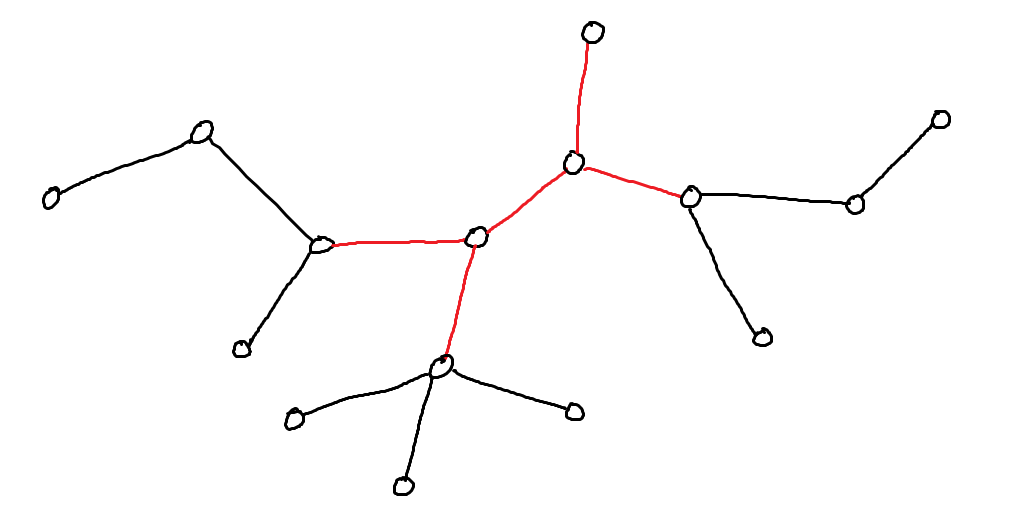
\includegraphics[scale=0.5]{stickbug.png}
\end{center}

위의 트리에는 서로 다른 자벌레가 총 $6$개 존재합니다.

입력으로 주어진 트리에 대해서, 트리에 존재하는 서로 다른 자벌레의 수를 구하는 프로그램을 작성해 주세요.